% !TEX root = ./main.tex
\begin{figure}[h]
    \centering
    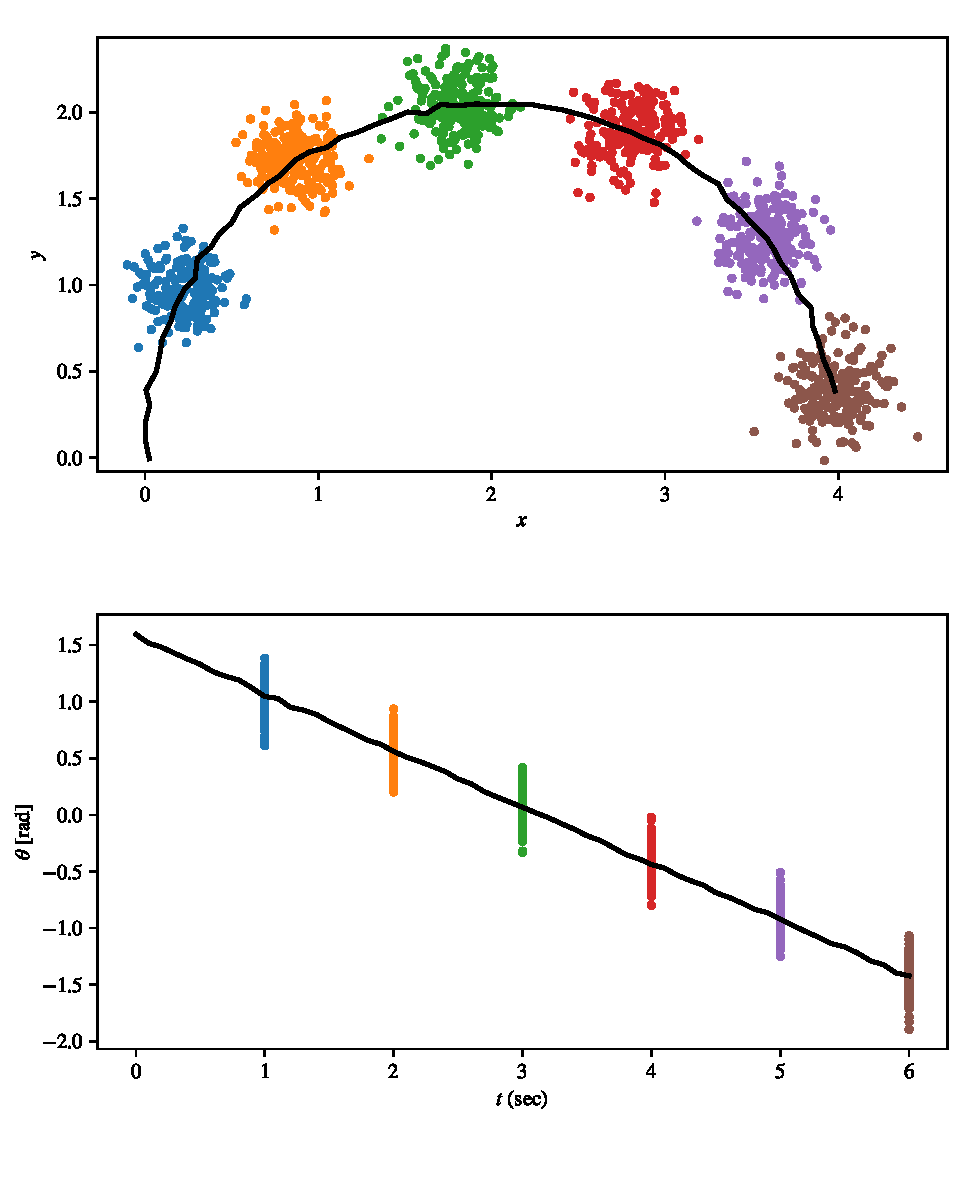
\includegraphics[width=0.8\textwidth]{q1_3.pdf}
    \vspace{-5mm}
    \caption{Particle filter for $N=200$ particles. Each color represents a snapshot of the particles at a particular time. The black line is the state estimate of $x$, $y$ and $\theta$ every $dt=0.1$ seconds.}
\end{figure}